\label{sec:viz-api}

We next describe the design of VizAPI, including details on how we
collect information and format it to the d3js visualization
library. We also describe two case studies showing potential uses of
VizAPI.

\begin{figure*}[h]
\begin{center}
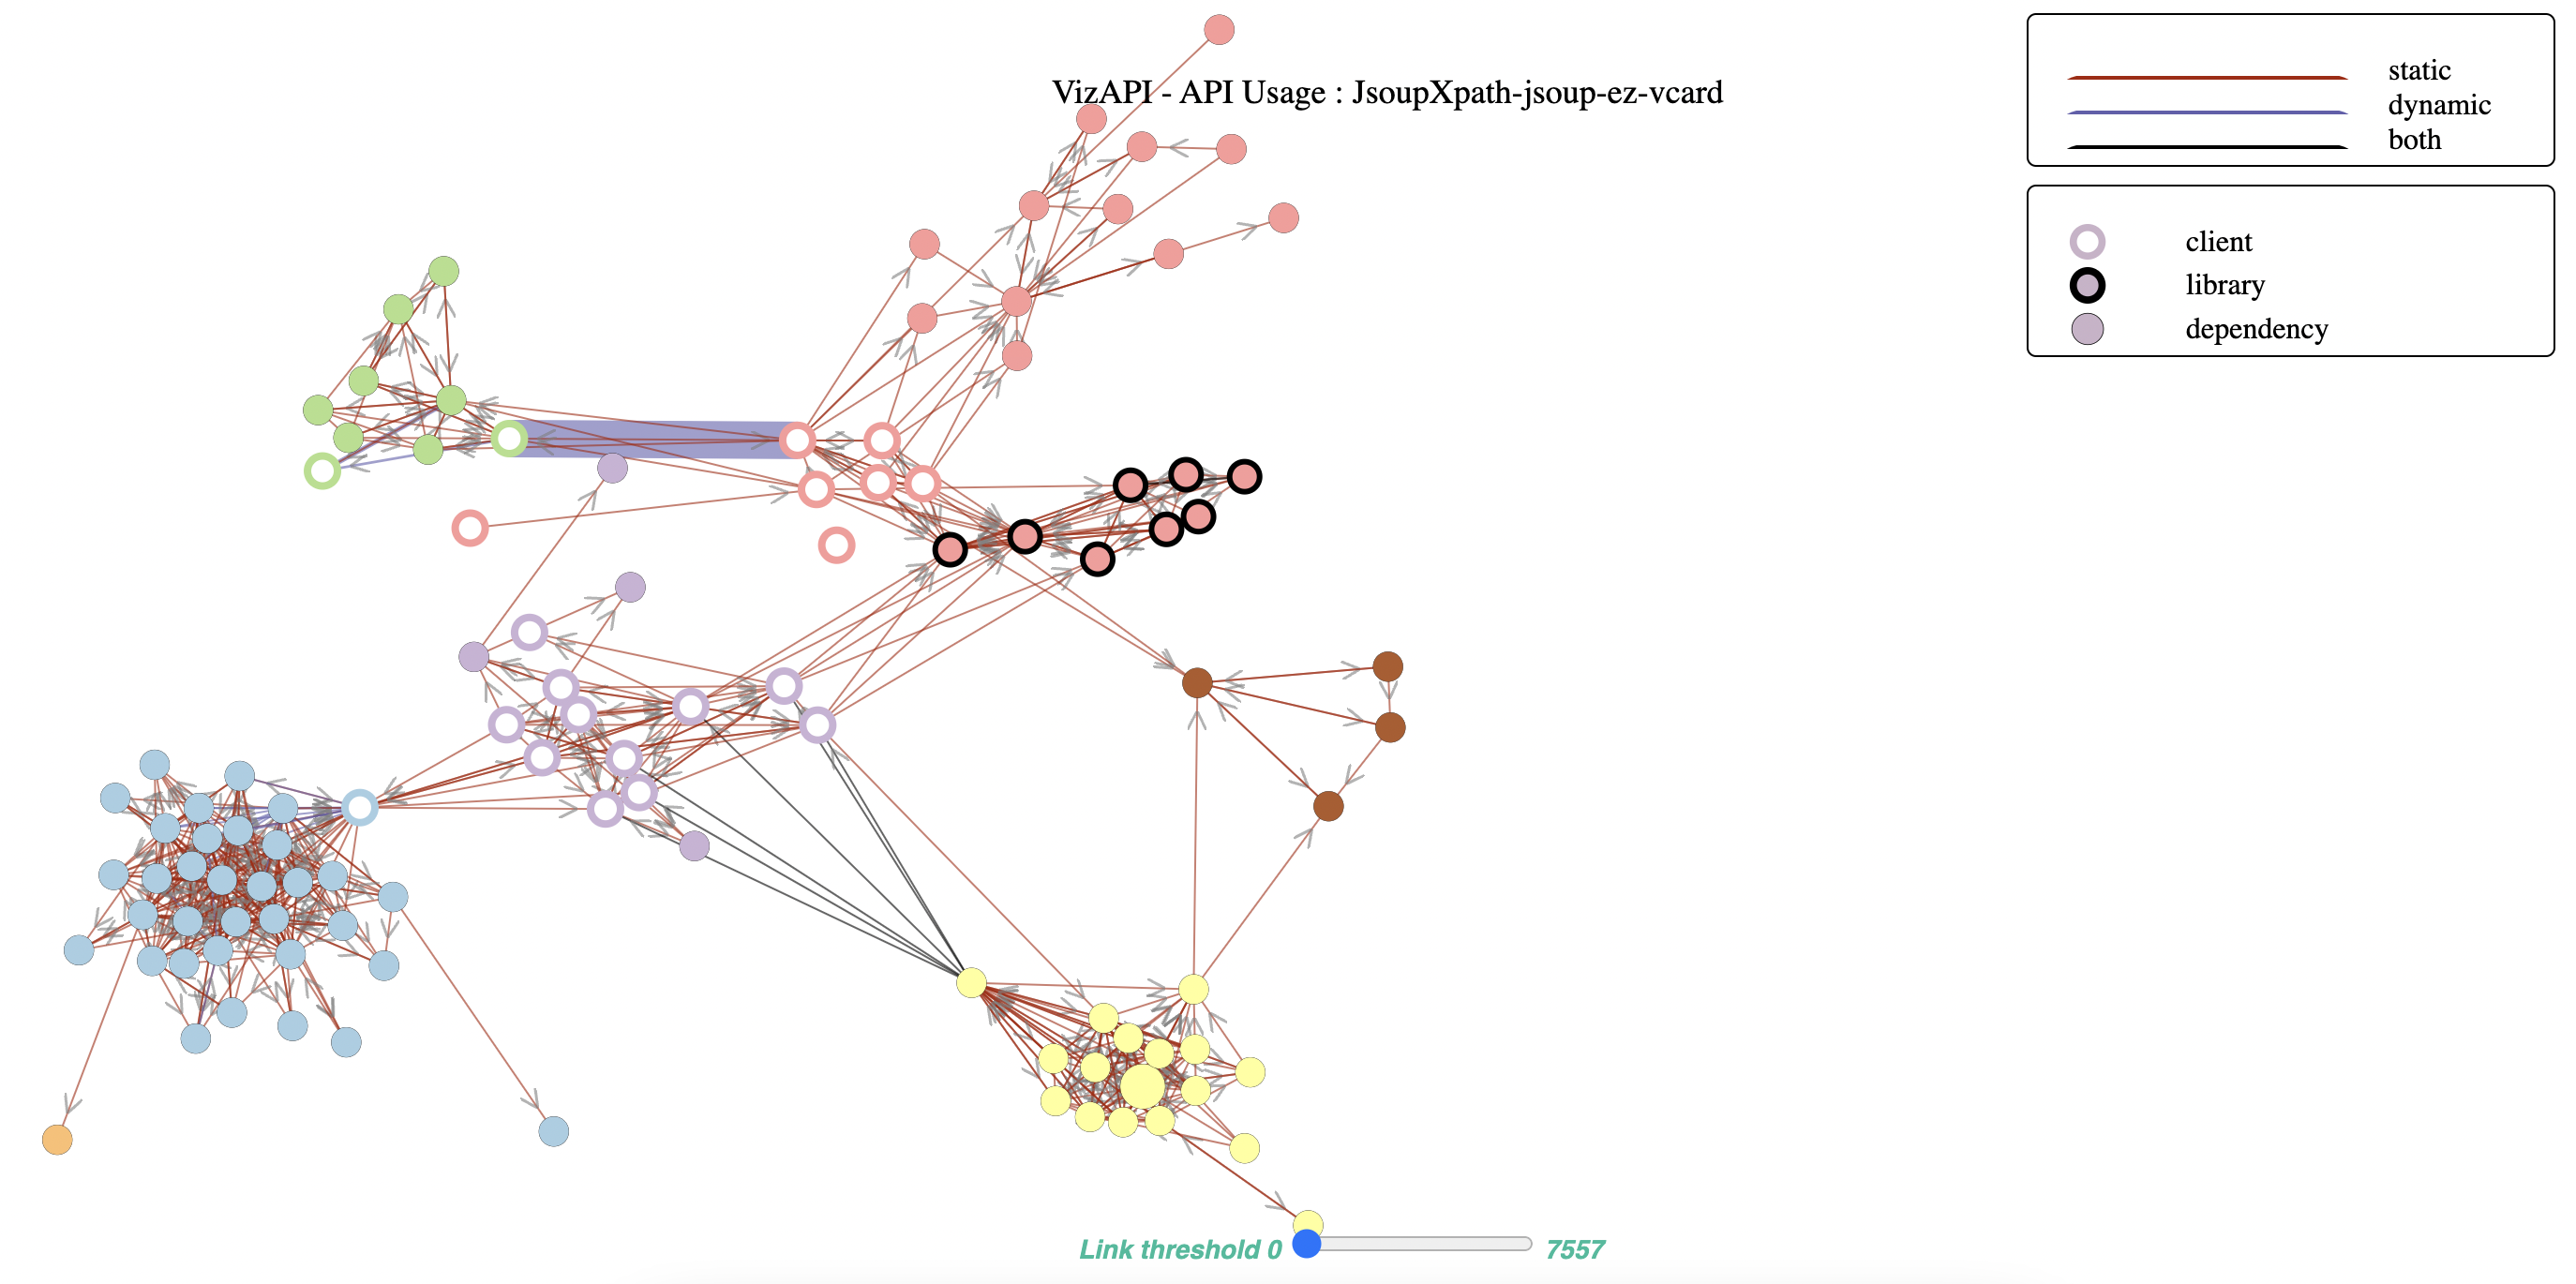
\includegraphics[scale=1,width=15cm,height=8cm]{images/usage-scenario1.png}
\caption{Usage Scenario 1: jsoup (library), JsoupXpath (client), ez-vcard (client)}
\label{fig:usagescenario1}
\end{center}
\end{figure*}

\subsection{Design}
\label{subsec:collecting-data}
Our goal is to visualize interactions between different software components---between
clients and libraries, and between libraries and other libraries. We now explain
how we collect static and dynamic information about software behaviour.
Figure~\ref{fig:workflow} summarizes our instrumentation and
data capture workflow. 

To identify interactions across the client/library boundaries,
we first inspect JAR files of each software component to obtain a list of
classes for every component. We then associate classes and their members to
components based on these lists.

\paragraph{Static information} We perform a static analysis to record
API uses, namely class hierarchy analysis. 

Using Javassist~\cite{chiba00:_load_struc_reflec_java}, we identify type
references which includes references at call sites, fields, annotations for 
classes, methods and fields, method parameters and casts. 

We then identify subtypes, also using Javassist, to determine possible 
interactions across client/library boundaries and library/library boundaries.

\paragraph{Dynamic information} We collect dynamic data by running client
test suites under instrumentation. 
The instrumentation records API
uses which cross client/library boundaries, as well as library/library boundaries
for libraries that are transitively used. We also use
Javassist to perform this
instrumentation and then use the build system of each project (Maven or Gradle) to run its
tests. 

\begin{figure*}[h]
 \begin{center}
\resizebox{0.7\textwidth}{!}{
  \begin{tikzpicture}
    \node[block] (client) {client};
    \node[block,below=1cm of client] (library) {library};

    \draw (library) -- node[left] (depends) {depends on} (client);

    \node[above left=.75em of client] (ja) {\begin{minipage}{7em} modify \\to use Javassist \end{minipage}};
    \draw[-Latex] (ja) -> (client);
    \draw[-Latex] (ja) to [->,bend right=35] (library.west);

    \node[block, above right=2em of client,xshift=-2em] (olib) {other library};
    \draw (client) -- node[right,xshift=.1em] (also) {also depends on} (olib);

    \node[oval,right=of depends] (test) {maven/gradle: run tests};

    \draw[-Latex] (client) to [->,bend left=15] (test);

    \node[block, right=10em of client] (output) {test output};
    \node[block, right=10em of library] (raw) {raw API usage info};

    \draw[-Latex] (test) to (output);
    \draw[-Latex] (test) to (raw);

    \node[oval, right=of raw] (Py) {Python scripts};
    \draw[-Latex] (raw) to (Py);

    \node[block, right=1em of Py] (viz) {D3 visualizations};
    \draw[-Latex] (Py) to (viz);
  \end{tikzpicture}
}
  \caption{Our instrumentation workflow. We modify existing project infrastructure to instrument clients and to run their test suites, producing raw data, which we process with our Python scripts to create D3 visualizations.}
  \label{fig:workflow}
 \end{center}
\end{figure*}

At every invoke instruction in every
loaded method which transfers control between the client and the
library, we add code to record that invoke by incrementing a counter.
We handle both static and virtual (including special, virtual,
interface, and dynamic) calls. Crossing the client/library boundary
includes callbacks from the library to the client as well as conventional
calls from the client to the library. 

We also record field accesses (direct and reflective), dynamic proxies
and reflective calls, Java annotations, implementations,
instantiations, and casts.

\subsection{Visualization System}
\label{subsec:vis-system}

Once we have generated data, we use a modified version
of the d3graph\footnote{\url{https://pypi.org/project/d3graph/}} library in Python to generate a d3js\footnote{\url{https://d3js.org/}}
visualization. 

VizAPI graphs are force-directed graphs based on the
frequency of interactions between different software components. 
Each software component can be one of: a client; a library; or a dependency.
Both libraries and dependencies refer to external libraries imported by components.
We refer to components used by clients as libraries, and components used by libraries
as dependencies. The graph in Figure~\ref{fig:usagescenario1}
is a graph produced by VizAPI.
Each node is a set of one or more packages (or classes or methods) 
that belong to the same JAR. We coalesce nodes if they originate from the same 
JAR file and have the same incoming and outgoing edges. Each edge is directed 
from the source package(s) to the target package(s) and represents an interaction 
(invocations, fields, annotations, subtyping) between packages. We run a 
clustering algorithm and use its output to colour nodes based on the cluster 
that they belong to, so a colour could include nodes from the same or different JARs.
Hovering on a node shows the list of packages and 
the JAR that they belong to, 
formatted as “jar : $<$space separated list of packages$>$”.

\subsection{Case Study}
\label{subsec:evaluation}

We conducted a pilot study of VizAPI on an 85-project subset of the
Duets benchmarks~\cite{durieux21}. Our study included 10 libraries and
their clients. For libraries, we pick the most popular Maven repositories 
in different categories such as logging and json parsing. We pick clients partly
from popular Github repositories and partly from Duets~\cite{durieux21}.
We collect both static and dynamic data for these projects.

\subsubsection{Usage Scenario 1: jsoup}
Now, we walk through an example usage scenario of VizAPI.
The graph in Figure~\ref{fig:usagescenario1} represents static and dynamic interactions of 2 clients with the jsoup\footnote{\url{https://github.com/jhy/jsoup}\label{jsoup}} library. Our clients are JsoupXpath\footnote{\url{https://github.com/zhegexiaohuozi/JsoupXpath}\label{jsoupxpath}} and ez-vcard\footnote{\url{https://github.com/mangstadt/ez-vcard}\label{ez-vcard}}.

We can start our exploration with the cluster of pink nodes. Many of these nodes belong to either JsoupXpath or jsoup. When we hover over them, the hover hints tell us that the client JsoupXpath calls directly into \texttt{org.jsoup.nodes} and \texttt{org.jsoup.select}. Notably, and as we might expect, we can see that \texttt{org.jsoup.helper} and \texttt{org.jsoup.internal} aren't called directly by JsoupXpath. This would mean that breaking changes in \texttt{org.jsoup.helper} or \texttt{org.jsoup.internal} wouldn't directly affect JsoupXpath\footnote{As a specific example, the retraction of an internal jsoup API would not break this client. Behavioural changes that are directly passed through to the external API, e.g. through delegation, can still break clients, but we can consider those to be changes in the external API.} 

Similarly, ez-vcard, which belongs to the purple cluster in Figure~\ref{fig:usagescenario1}, directly calls into \texttt{org.jsoup}. ez-vcard also calls into jackson-core\footnote{\url{https://github.com/FasterXML/jackson-core}\label{jackson-core}} and jackson-databind\footnote{\url{https://github.com/FasterXML/jackson-databind}\label{jackson-databind}}, which are very tightly coupled amongst their own packages and with each other. This could mean that breaking changes in these libraries can propagate to many of their own packages.

\subsubsection{Usage Scenario 2: dataprocessor}
\begin{figure*}[h]
\begin{center}
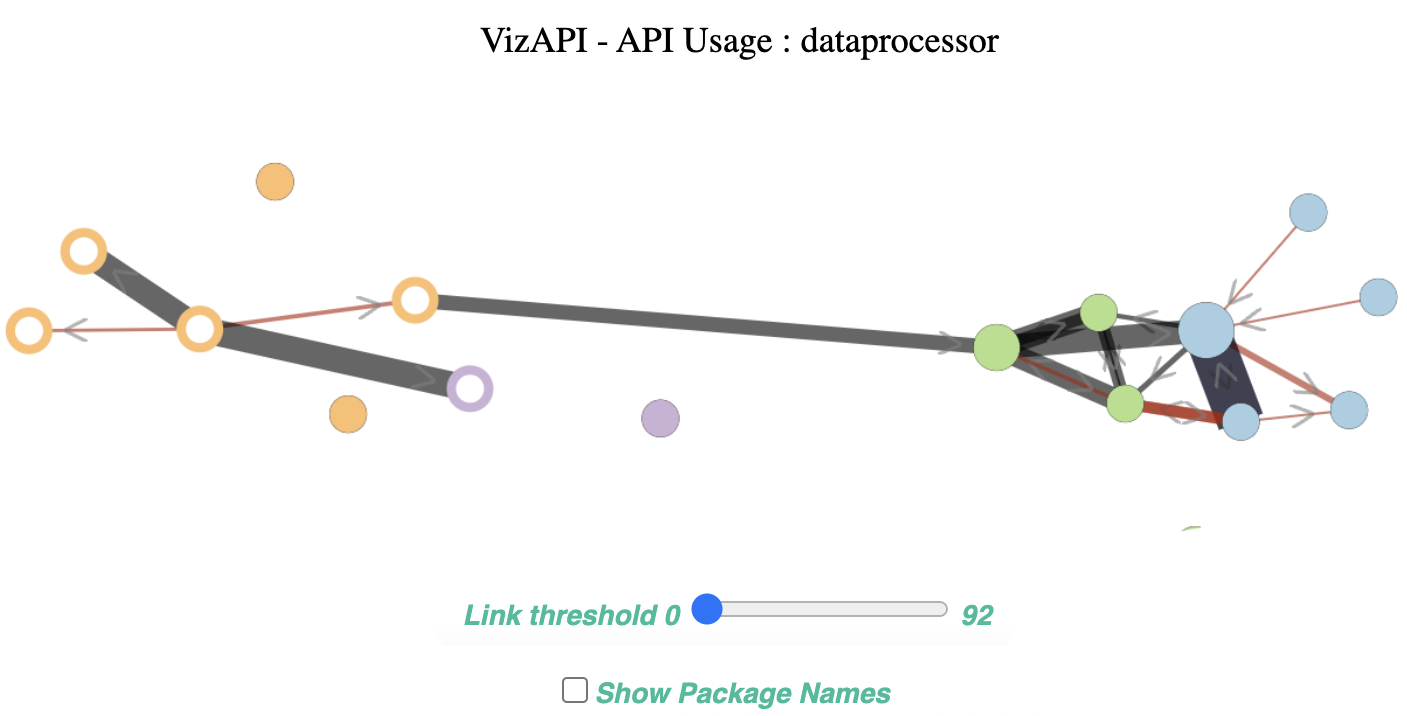
\includegraphics[scale=1,width=9cm,height=8cm]{images/usage-scenario2.png}
\caption{Usage Scenario 1: dataprocessor (client)}
\label{fig:usagescenario2}
\end{center}
\end{figure*}

Figure~\ref{fig:usagescenario2} presents a second usage scenario. Here, we focus on a client, dataprocessor\footnote{\url{https://github.com/dadiyang/dataprocessor}\label{dataprocessor}}. This client uses the fastjson\footnote{\url{https://github.com/alibaba/fastjson}\label{fastjson}} library. Our visualization shows calls only from dataprocessor package \texttt{com.github.dataprocessor.slice}, which is the orange client node (identity of the package available from clicking on the orange node) to the package \texttt{com.alibaba.fastjson}. No other parts of dataprocessor use fastjson. This means that when dataprocessor needs to upgrade its fastjson version, the dataprocessor developers only need to inspect the source code in the \texttt{com.github.dataprocessor.slice} package. 

Note also the disconnected nodes in Figure~\ref{fig:usagescenario2}. These are all packages of fastjson that are unused by dataprocessor: any breaking changes in these packages definitely do not directly affect dataprocessor, and are less likely to affect it overall than packages that are directly used.
